\documentclass{problemset}
\usepackage{amsmath}

\usepackage{lipsum}
%\usepackage{showframe}
%\usepackage{layout}


\usepackage[charter,cal=cmcal]{mathdesign} %different font
\usepackage{microtype}
\usepackage{mathtools}
%\usepackage{amsfonts}
%\usepackage{amssymb}
\usepackage{graphicx}
\usepackage[inline]{enumitem}
\usepackage{xparse}
\usepackage{ifthen}
\usepackage{graphicx}
\usepackage{caption}
\usepackage{subcaption}
\usepackage{color}
\usepackage{tikz}
\usepackage{fancyhdr}
\usepackage{calc}
\usepackage{wrapfig}
\usepackage{marginnote}
\usepackage{mparhack}
\usepackage{marginfix}
\usepackage[hidelinks]{hyperref}


\usepackage{pgfplots}
\pgfplotsset{compat=newest}
%%%
% Useful Linear Algebra macros
%%%
\newcommand{\declarecommand}[1]{\providecommand{#1}{}\renewcommand{#1}}
\declarecommand{\R}{\mathbb{R}}  % we don't care if it's already defined.  We really want *this* command!
\declarecommand{\Z}{\mathbb{Z}}
\declarecommand{\Q}{\mathbb{Q}}
\declarecommand{\N}{\mathbb{N}}
\declarecommand{\C}{\mathbb{C}}
\declarecommand{\d}{\mathrm{d}}
\declarecommand{\dd}{\mathbbm{d}} % exterior derivative
\DeclareMathOperator{\Span}{span}
\DeclareMathOperator{\Img}{img}
\DeclareMathOperator{\Id}{id}
\DeclareMathOperator{\Range}{range}
\DeclareMathOperator{\Rref}{rref}
\DeclareMathOperator{\Rank}{rank}
\DeclareMathOperator{\Comp}{comp}
\DeclareMathOperator{\Null}{null}
\DeclareMathOperator{\Nullity}{nullity}
\DeclareMathOperator{\Char}{char}
\DeclareMathOperator{\Proj}{proj}
\DeclareMathOperator{\Flux}{Flux}
\DeclareMathOperator{\Circ}{Circ}
\DeclareMathOperator{\chr}{char}
\DeclareMathOperator{\Dim}{dim}
\DeclareMathOperator{\Perp}{perp}
\DeclareMathOperator{\Ker}{kernel}
\DeclareMathOperator{\Row}{row}
\DeclareMathOperator{\Col}{col}
\newcommand{\proj}{\Proj}
\newcommand{\rref}{\Rref}
\newcommand{\xhat}{{\hat {\mathbf x}}}
\newcommand{\yhat}{{\hat {\mathbf y}}}
\newcommand{\zhat}{{\hat {\mathbf z}}}
\newcommand{\mat}[1]{\begin{bmatrix*}[r]#1\end{bmatrix*}}
\newcommand{\matc}[1]{\begin{bmatrix}#1\end{bmatrix}}
\newcommand{\formarg}[2]{\big(#1;\, #2\big)}
\DeclarePairedDelimiter\abs{\lvert}{\rvert}
\DeclarePairedDelimiter\Abs{\lvert}{\rvert}
\DeclarePairedDelimiter\norm{\lVert}{\rVert}
% just to make sure it exists
\providecommand\given{}
% can be useful to refer to this outside \Set
\newcommand\SetSymbol[1][]{%
	\nonscript\::%
	\allowbreak
	\nonscript\:
	\mathopen{}}
\DeclarePairedDelimiterX\Set[1]\{\}{%
	\renewcommand\given{\SetSymbol[\delimsize]}
	#1
}

%\tcbuselibrary{skins}
%\usetikzlibrary{shadings}


%%%
% Set up the margins to use a fairly large area of the page
%%%
%\textwidth=5.2in
%\topmargin=-1in
%\textheight=10in
%\parskip=.07in
%\parindent=0in


\fancypagestyle{siefken}{%
	\rfoot{\footnotesize\it \copyright\,Jason Siefken, 2015--2018 \ \makebox(30,5){
\includegraphics[height=1.2em]{by-sa.pdf}}}
	\lfoot{}
	\renewcommand{\headrulewidth}{0pt}
}
\fancypagestyle{iola}{%
	\rfoot{\footnotesize\it \copyright\,IOLA Team \url{iola.math.vt.edu} \ \makebox(30,5){
\includegraphics[height=2.2em]{images/iolalogo.png}}}
	\lfoot{}
	\renewcommand{\headrulewidth}{0pt}
}

\DeclareDocumentEnvironment{iola}{o}{%
	\newpage
	\pagestyle{iola}
}{%
	\newpage
}



\begin{document}
\begin{iola}
\section*{Task 1.1: The Magic Carpet Ride}
\addcontentsline{toc}{subsection}{Task 1.1: The Magic Carpet Ride}

You are a young traveler, leaving home for the first time. Your parents
want to help you on your journey, so just before your departure, they give you two
gifts. Specifically, they give you two forms of transportation: a hover board and
a magic carpet. Your parents inform you that both the hover board and the magic carpet
have restrictions in how they operate: 

\begin{minipage}{\textwidth}
	\vspace{.5cm}
	\begin{wrapfigure}{l}{1in}
	\vspace{-.8cm}
	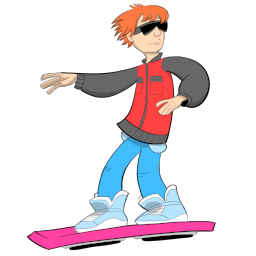
\includegraphics[width=1in]{images/HoverBoard-small.png}
	\end{wrapfigure}

	We denote the restriction on the hover board's movement by the vector
	$\mat{3 \\1}$. By this we mean that if
	the hover board traveled ``forward'' for one hour, it would move along a
	``diagonal'' path that would result in a displacement of 3 miles East and
	1 mile North of its starting location.
\end{minipage}

\begin{minipage}{\textwidth}
	\vspace{.5cm}
	\begin{wrapfigure}{l}{1in}
	\vspace{-.8cm}
	
\includegraphics[width=1in]{images/MagicCarpet-small.png}
	\end{wrapfigure}

	We denote the restriction on the magic carpet's movement by the vector
	$\mat{1 \\2 }$. By this we mean that if the
	magic carpet traveled ``forward'' for one hour, it would move along a
	``diagonal'' path that would result in a displacement of 1 mile East and
	2 miles North of its starting location.
\end{minipage}

\lfoot{\footnotesize Drawings by \url{@DavidsonJohnR} (twitter)}

\vspace{10mm}

% Scenario Section
\textbf{Scenario One: The Maiden Voyage}

Your Uncle Cramer suggests that your first adventure should be to go visit
the wise man, Old Man Gauss. Uncle Cramer tells you that Old Man Gauss
lives in a cabin that is 107 miles East and 64 miles North of your home.

\vspace{5mm}

\textbf{Task:}
\par
Investigate whether or not you can use the hover board and the magic
carpet to get to Gauss's cabin. If so, how? If it is not possible to
get to the cabin with these modes of transportation, why is that the case?

%\vspace{5mm}
% As a group, state and explain your answer(s) on the group whiteboard. Use
% the vector notation for each mode of transportation as part of your
% explanation and use a diagram or graphic to help illustrate your
% point(s).
\end{iola}

\begin{iola}
\section*{Task 1.2: The Magic Carpet Ride, Hide and Seek}
\addcontentsline{toc}{subsection}{Task 1.2: The Magic Carpet Ride, Hide and Seek}


You are a young traveler, leaving home for the first time. Your parents
want to help you on your journey, so just before your departure, they give
you two gifts. Specifically, they give you two forms of transportation:
a hover board and a magic carpet. Your parents inform you that both the
hover board and the magic carpet have restrictions in how they operate:



\begin{minipage}{\textwidth}
	\vspace{.5cm}
	\begin{wrapfigure}{l}{1in}
	\vspace{-.8cm}
	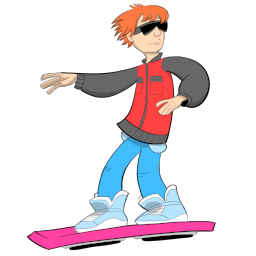
\includegraphics[width=1in]{images/HoverBoard-small.png}
	\end{wrapfigure}

	We denote the restriction on the hover board's movement by the vector
	$\mat{3 \\1}$. By this we mean that if
	the hover board traveled ``forward'' for one hour, it would move along a
	``diagonal'' path that would result in a displacement of 3 miles East and
	1 mile North of its starting location.
\end{minipage}

\begin{minipage}{\textwidth}
	\vspace{.5cm}
	\begin{wrapfigure}{l}{1in}
	\vspace{-.8cm}
	
\includegraphics[width=1in]{images/MagicCarpet-small.png}
	\end{wrapfigure}

	We denote the restriction on the magic carpet's movement by the vector
	$\mat{1 \\2 }$. By this we mean that if the
	magic carpet traveled ``forward'' for one hour, it would move along a
	``diagonal'' path that would result in a displacement of 1 mile East and
	2 miles North of its starting location.
	\vspace{1cm}
\end{minipage}



\textbf{Scenario Two: Hide-and-Seek}

Old Man Gauss wants to move to a cabin in a different location. You are
not sure whether Gauss is just trying to test your wits at finding him
or if he actually wants to hide somewhere that you can't visit him.

\vspace{5mm}

\textbf{Are there some locations that he can hide and you cannot reach him
with these two modes of transportation?}

Describe the places that you
can reach using a combination of the hover board and the magic carpet and
those you cannot. Specify these geometrically and algebraically. Include
a symbolic representation using vector notation. Also, include a convincing
argument supporting your answer.

%\vspace{5mm} \par \textbf{Use your
%group's whiteboard as a space to write out our work as your work together
%on this problem.}
\end{iola}

\begin{iola}
\section*{Task 1.3: The Magic Carpet, Getting Back Home}
\addcontentsline{toc}{subsection}{Task 1.3: The Magic Carpet Ride, Getting Back Home}

Suppose you are now in a three-dimensional world for the carpet
ride problem, and you have three modes of transportation:
\[
	\vec v_1 = \mat{1 \\1 \\ 1}\qquad
	\vec v_2 = \mat{6 \\3 \\ 8}\qquad
	\vec v_3 = \mat{4 \\1 \\ 6}
\]

You are only allowed to use each mode of transportation \textbf{once}
(in the forward or backward direction) for a fixed amount of time ($c_1$
on $\vec v_1$, $c_2$ on $\vec v_2$, $c_3$ on $\vec v_3$).

\vspace{5mm}


\begin{enumerate}
	\item  Find the amounts of time on each mode of transportation ($c_1$, $c_2$, 
		and $c_3$, respectively) needed to go on a journey that starts and ends 
		at home \emph{or} explain why it is not possible to do so.

	\item Is there more than one way to make a journey that meets the
		requirements described above? (In other words, are there different
		combinations of times you can spend on the modes of transportation so
		that you can get back home?) If so, how?

	\item Is there anywhere in this 3D world that Gauss
		could hide from you? If so, where? If not, why not?

	\item What is $\Span\Set*{\mat{1\\1\\1},\mat{6\\3\\8},\mat{4\\1\\6}}$?

\end{enumerate}
\end{iola}
\begin{iola}
\section*{Task 1.4: Linear Independence and Dependence, Creating Examples}
\addcontentsline{toc}{subsection}{Task 1.4: Linear Independence and Dependence, Creating Examples}



\begin{enumerate}
	\item Fill in the following chart keeping track of the strategies you used to generate
examples.

\vspace{2mm}

\begin{center}
\begin{tabular}{|c|c|c|}
	\hline
	&Linearly independent & Linearly dependent \\
	\hline
	A set of 2 vectors in $\R^2$ &&\\
	\hline
	A set of 3 vectors in $\R^2$ &&\\
	\hline
	A set of 2 vectors in $\R^3$ &&\\
	\hline
	A set of 3 vectors in $\R^3$ &&\\
	\hline
	A set of 4 vectors in $\R^3$ &&\\
	\hline
\end{tabular}
\end{center}
	
		\item Write at least two generalizations that can
			be made from these examples and the strategies you
			used to create them.

\end{enumerate}

\end{iola}
\begin{iola}
\section*{Task 2.1: Italicizing N}
\addcontentsline{toc}{subsection}{Task 2.1: Italicizing N}

\hfill\begin{tikzpicture}[scale=1.5]
    \begin{axis}[
		    axis equal image,
		    axis line style={draw=none},
		    tick style={draw=none},
		    yticklabels={,,},
		    xticklabels={,,},
		 xmin=-.5,
		 xmax=3.5,
		 ymin=-.5,
		 ymax=5.5,
		 major grid style={dotted, gray, thick},
                 xtick={0,1,2,3},
		 ytick={0,1,2,3,4,5},
                 grid=both]

	 \draw[black, thick] (0,0) -- (0,3) -- (2,0) -- (2,3);
    \end{axis}
\end{tikzpicture}\hfill
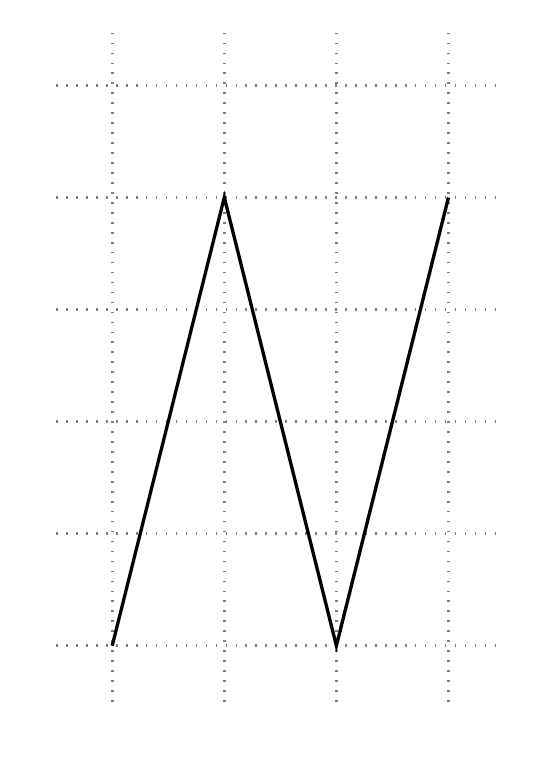
\begin{tikzpicture}[scale=1.5]
    \begin{axis}[
		    axis equal image,
		    axis line style={draw=none},
		    tick style={draw=none},
		    yticklabels={,,},
		    xticklabels={,,},
		 xmin=-.5,
		 xmax=3.5,
		 ymin=-.5,
		 ymax=5.5,
		 major grid style={dotted, gray, thick},
                 xtick={0,1,2,3},
		 ytick={0,1,2,3,4,5},
                 grid=both]

	 \draw[black, thick] (0,0) -- (1,4) -- (2,0) -- (3,4);
    \end{axis}
\end{tikzpicture}\hfill

Suppose that the ``N'' on the left is written in regular 12-point font.  Find a matrix $A$ that will transform
	the ``N'' into the letter on the right which is written in an \emph{italic} 16-point font.

Work with your group to write out your solution and approach.  Make a list of any assumptions you
notice your group making or any questions for further pursuit.
\end{iola}
\begin{iola}
\section*{Task 2.2: Beyond the N}
\addcontentsline{toc}{subsection}{Task 2.2: Beyond the N}

	A few students were wondering how letters placed in other
locations in the plane would be transformed under $A= \mat{ 1&  1/3  \\ 0 & 4/3}$. 
	If an ``E'' is placed around the
	``N,'' the students argued over four different possible results for the
	transformed E's. Which choice below, if any, is correct, and why? If none of
	the four options are correct, what would the correct option be, and why?



\begin{minipage}{6.5in}
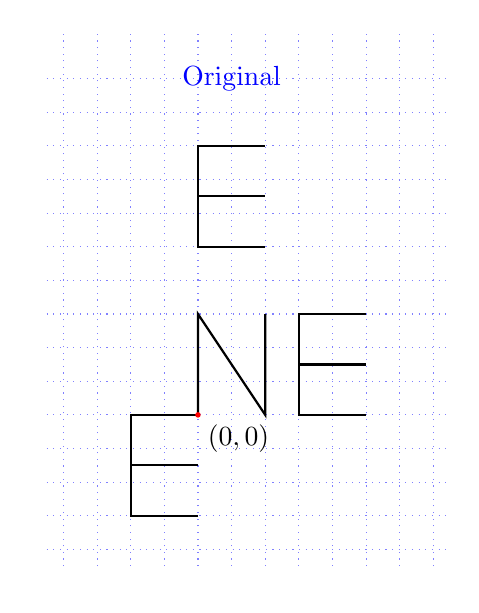
\begin{tikzpicture}
    \begin{axis}[scale=1.2,
		    axis equal image,
		    axis line style={draw=none},
		    tick style={draw=none},
		    yticklabels={,,},
		    xticklabels={,,},
		 xmin=-4.5,
		 xmax=7.5,
		 ymin=-4.5,
		 ymax=11.5,
		 major grid style={dotted, blue!50!white},
                 xtick={-10,-9,...,10},
                 ytick={-10,-9,...,10},
                 grid=both]
	 \draw[black, thick] (0,0) -- (0,3) -- (2,0) -- (2,3);

	 \draw[black, thick] (0,0) -- (-2,0) -- (-2,-3) -- (0,-3)(-2,-1.5) -- (0,-1.5);

	\draw[black, thick] (5, 3) -- (3, 3) -- (3, 0) -- (5, 0)  (3, 1.5) -- (5, 1.5);
	    \draw[black, thick] (2, 8) -- (0, 8) -- (0, 5) -- (2, 5)  (0, 6.5) -- (2, 6.5);

	    \node[blue] at (1,10) {Original};
	    \fill[red] (0,0) circle[radius=1pt] node[below right, black] {$(0,0)$};

    \end{axis}
\end{tikzpicture}
\hfill
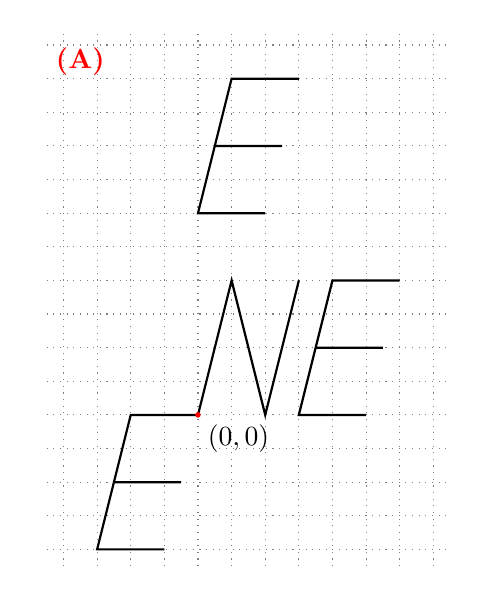
\begin{tikzpicture}
    \begin{axis}[scale=1.2,
		    axis equal image,
		    axis line style={draw=none},
		    tick style={draw=none},
		    yticklabels={,,},
		    xticklabels={,,},
		 xmin=-4.5,
		 xmax=7.5,
		 ymin=-4.5,
		 ymax=11.5,
		 major grid style={dotted, gray},
                 xtick={-10,-9,...,10},
                 ytick={-10,-9,...,11},
                 grid=both]
	\draw[black, thick] (0, 0) -- (1, 4) -- (2, 0) -- (3, 4);

	\draw[black, thick] (-1, -4) -- (-3, -4) -- (-2, 0) -- (0, 0)  (-2.5, -2) -- (-0.5, -2);
	\draw[black, thick] (5, 0) -- (3, 0) -- (4, 4) -- (6, 4) (3.5, 2) -- (5.5, 2);
	\draw[black, thick](2, 6) -- (0, 6) -- (1, 10) -- (3, 10) (0.5, 8) -- (2.5, 8) ;
	    \node[red] at (-3.5,10.5) {\bfseries (A)};
	    \fill[red] (0,0) circle[radius=1pt] node[below right, black] {$(0,0)$};
    \end{axis}
\end{tikzpicture}
\hfill
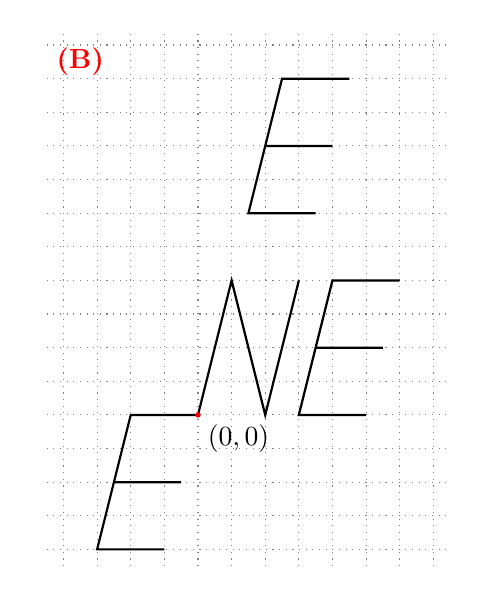
\begin{tikzpicture}
    \begin{axis}[scale=1.2,
		    axis equal image,
		    axis line style={draw=none},
		    tick style={draw=none},
		    yticklabels={,,},
		    xticklabels={,,},
		 xmin=-4.5,
		 xmax=7.5,
		 ymin=-4.5,
		 ymax=11.5,
		 major grid style={dotted, gray},
                 xtick={-10,-9,...,10},
                 ytick={-10,-9,...,11},
                 grid=both]
	\draw[black, thick] (0, 0) -- (1, 4) -- (2, 0) -- (3, 4);

	\draw[black, thick] (-1, -4) -- (-3, -4) -- (-2, 0) -- (0, 0)  (-2.5, -2) -- (-0.5, -2);
	\draw[black, thick] (5, 0) -- (3, 0) -- (4, 4) -- (6, 4) (3.5, 2) -- (5.5, 2);
	\draw[black, thick] (3.5, 6) -- (1.5, 6) -- (2.5, 10) -- (4.5, 10) (2.0, 8) -- (4.0, 8);
	    \node[red] at (-3.5,10.5) {\bfseries (B)};
	    \fill[red] (0,0) circle[radius=1pt] node[below right, black] {$(0,0)$};
    \end{axis}
\end{tikzpicture}
\end{minipage}
\hfill

\hfill
\begin{minipage}{6.5in}
	\hspace{2.13in}
	\hfill
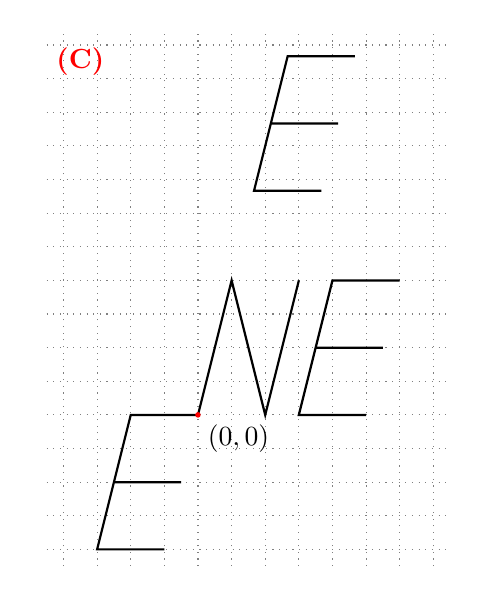
\begin{tikzpicture}
    \begin{axis}[scale=1.2,
		    axis equal image,
		    axis line style={draw=none},
		    tick style={draw=none},
		    yticklabels={,,},
		    xticklabels={,,},
		 xmin=-4.5,
		 xmax=7.5,
		 ymin=-4.5,
		 ymax=11.5,
		 major grid style={dotted, gray},
                 xtick={-10,-9,...,10},
                 ytick={-10,-9,...,11},
                 grid=both]
	\draw[black, thick] (0, 0) -- (1, 4) -- (2, 0) -- (3, 4);

	\draw[black, thick] (-1, -4) -- (-3, -4) -- (-2, 0) -- (0, 0)  (-2.5, -2) -- (-0.5, -2);
	\draw[black, thick] (5, 0) -- (3, 0) -- (4, 4) -- (6, 4) (3.5, 2) -- (5.5, 2);
	\draw[black, thick] (3.666666666666667, 6.666666666666667) -- (1.6666666666666667, 6.666666666666667) -- (2.666666666666667, 10.666666666666668) -- (4.666666666666667, 10.666666666666668)  (2.166666666666667, 8.666666666666668) -- (4.166666666666667, 8.666666666666668);
	    \node[red] at (-3.5,10.5) {\bfseries (C)};
	    \fill[red] (0,0) circle[radius=1pt,fill=blue] node[below right, black] {$(0,0)$};
    \end{axis}
\end{tikzpicture}
\hfill
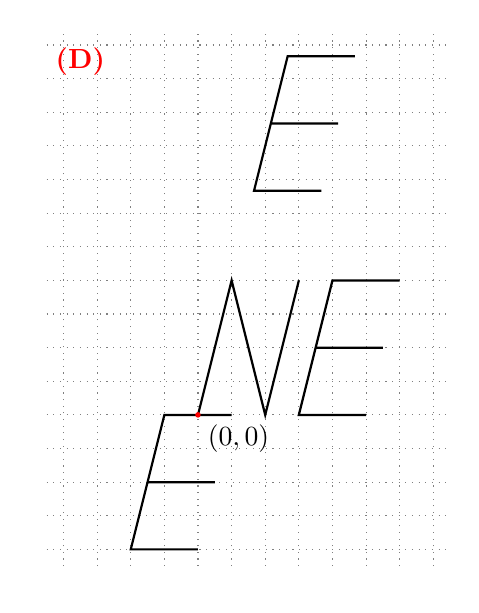
\begin{tikzpicture}
    \begin{axis}[scale=1.2,
		    axis equal image,
		    axis line style={draw=none},
		    tick style={draw=none},
		    yticklabels={,,},
		    xticklabels={,,},
		 xmin=-4.5,
		 xmax=7.5,
		 ymin=-4.5,
		 ymax=11.5,
		 major grid style={dotted, gray},
                 xtick={-10,-9,...,10},
                 ytick={-10,-9,...,11},
                 grid=both]
	\draw[black, thick] (0, 0) -- (1, 4) -- (2, 0) -- (3, 4);

	\draw[black, thick] (0, -4) -- (-2, -4) -- (-1, 0) -- (1, 0)  (-1.5, -2) -- (0.5, -2);
	\draw[black, thick] (5, 0) -- (3, 0) -- (4, 4) -- (6, 4) (3.5, 2) -- (5.5, 2);
	\draw[black, thick] (3.666666666666667, 6.666666666666667) -- (1.6666666666666667, 6.666666666666667) -- (2.666666666666667, 10.666666666666668) -- (4.666666666666667, 10.666666666666668)  (2.166666666666667, 8.666666666666668) -- (4.166666666666667, 8.666666666666668);
	    \node[red] at (-3.5,10.5) {\bfseries (D)};
	    \fill[red] (0,0) circle[radius=1pt,fill=blue] node[below right, black] {$(0,0)$};
    \end{axis}
\end{tikzpicture}
\end{minipage}
\hfill
\vfill
\end{iola}
\begin{iola}
\section*{Task 2.3: Pat and Jamie}
\addcontentsline{toc}{subsection}{Task 2.3: Pat and Jamie}

\begin{minipage}{.5\textwidth}
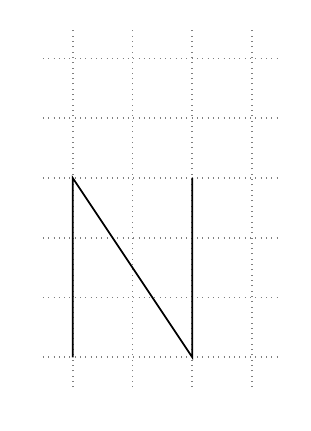
\begin{tikzpicture}[scale=.8]
    \begin{axis}[
		    axis equal image,
		    axis line style={draw=none},
		    tick style={draw=none},
		    yticklabels={,,},
		    xticklabels={,,},
		 xmin=-.5,
		 xmax=3.5,
		 ymin=-.5,
		 ymax=5.5,
		 major grid style={dotted, gray, thick},
                 xtick={0,1,2,3},
		 ytick={0,1,2,3,4,5},
                 grid=both]

	 \draw[black, thick] (0,0) -- (0,3) -- (2,0) -- (2,3);
    \end{axis}
\end{tikzpicture}\hfill
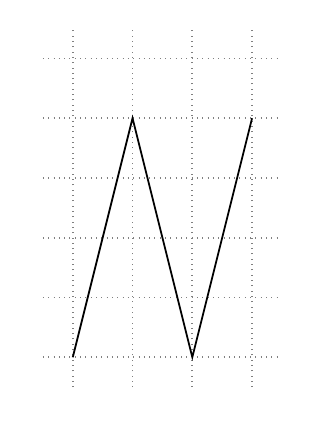
\begin{tikzpicture}[scale=.8]
    \begin{axis}[
		    axis equal image,
		    axis line style={draw=none},
		    tick style={draw=none},
		    yticklabels={,,},
		    xticklabels={,,},
		 xmin=-.5,
		 xmax=3.5,
		 ymin=-.5,
		 ymax=5.5,
		 major grid style={dotted, gray, thick},
                 xtick={0,1,2,3},
		 ytick={0,1,2,3,4,5},
                 grid=both]

	 \draw[black, thick] (0,0) -- (1,4) -- (2,0) -- (3,4);
    \end{axis}
\end{tikzpicture}\hfill
\end{minipage}
\begin{minipage}{.5\textwidth}

Suppose that the ``N'' on the left is written in regular 12-point font.  Find a matrix $A$ that will transform
	the ``N'' into the letter on the right which is written in an \emph{italic} 16-point font.
\end{minipage}

Two students---Pat and Jamie---explained their approach to the Italicizing N task as follows:
\begin{quote}\itshape
	In order to find the matrix $A$, we are going to find a matrix that makes the ``N'' taller,
	find a matrix that italicizes the taller ``N,'' and a combination of those two matrices
	will give the desired matrix $A$.
\end{quote}

\begin{enumerate}
	\item Do you think Pat and Jamie's approach allowed them to find $A$?  If so, do
		you think they found the same matrix that you did during Italicising N?
	\item Try Pat and Jamie's approach.  Either (a) come up with a matrix $A$ using
		their approach, or (b) explain why their approach does not work.
\end{enumerate}

\end{iola}

\begin{iola}
\section*{Task 2.4: Getting back N}
\addcontentsline{toc}{subsection}{Task 2.4: Getting back N}

\begin{minipage}{.5\textwidth}
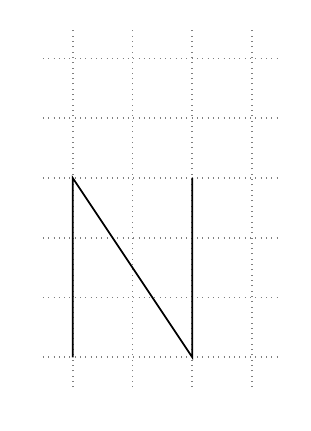
\begin{tikzpicture}[scale=.8]
    \begin{axis}[
		    axis equal image,
		    axis line style={draw=none},
		    tick style={draw=none},
		    yticklabels={,,},
		    xticklabels={,,},
		 xmin=-.5,
		 xmax=3.5,
		 ymin=-.5,
		 ymax=5.5,
		 major grid style={dotted, gray, thick},
                 xtick={0,1,2,3},
		 ytick={0,1,2,3,4,5},
                 grid=both]

	 \draw[black, thick] (0,0) -- (0,3) -- (2,0) -- (2,3);
    \end{axis}
\end{tikzpicture}\hfill
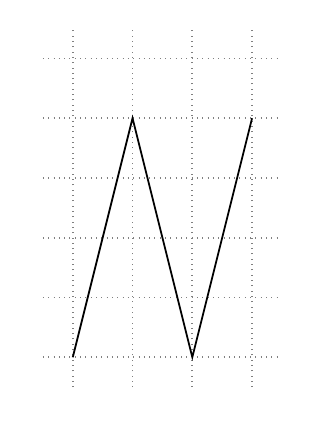
\begin{tikzpicture}[scale=.8]
    \begin{axis}[
		    axis equal image,
		    axis line style={draw=none},
		    tick style={draw=none},
		    yticklabels={,,},
		    xticklabels={,,},
		 xmin=-.5,
		 xmax=3.5,
		 ymin=-.5,
		 ymax=5.5,
		 major grid style={dotted, gray, thick},
                 xtick={0,1,2,3},
		 ytick={0,1,2,3,4,5},
                 grid=both]

	 \draw[black, thick] (0,0) -- (1,4) -- (2,0) -- (3,4);
    \end{axis}
\end{tikzpicture}\hfill
\end{minipage}
\begin{minipage}{.5\textwidth}

Suppose that the ``N'' on the left is written in regular 12-point font.  Find a matrix $A$ that will transform
	the ``N'' into the letter on the right which is written in an \emph{italic} 16-point font.
\end{minipage}

Two students---Pat and Jamie---explained their approach to the Italicizing N task as follows:
\begin{quote}\itshape
	In order to find the matrix $A$, we are going to find a matrix that makes the ``N'' taller,
	find a matrix that italicizes the taller ``N,'' and a combination of those two matrices
	will give the desired matrix $A$.
\end{quote}

Consider the new task: find a matrix $C$ that transforms the ``N'' on the right to
the ``N'' on the left.
\begin{enumerate}
	\item Use any method you like to find $C$.
	\item Use a method similar to Pat and Jamie's method, only use it to find $C$ instead
		of $A$.
\end{enumerate}
\end{iola}


\begin{iola}
\section*{Task 3.1: The Green and the Black}
\addcontentsline{toc}{subsection}{Task 3.1: The Green and the Black}
Consider the following two bases for $\R^2$: the green basis $\mathcal G=\{\vec g_1,\vec g_2\}$
and the black basis $\mathcal B=\{\vec e_1,\vec e_2\}$.
\begin{center}
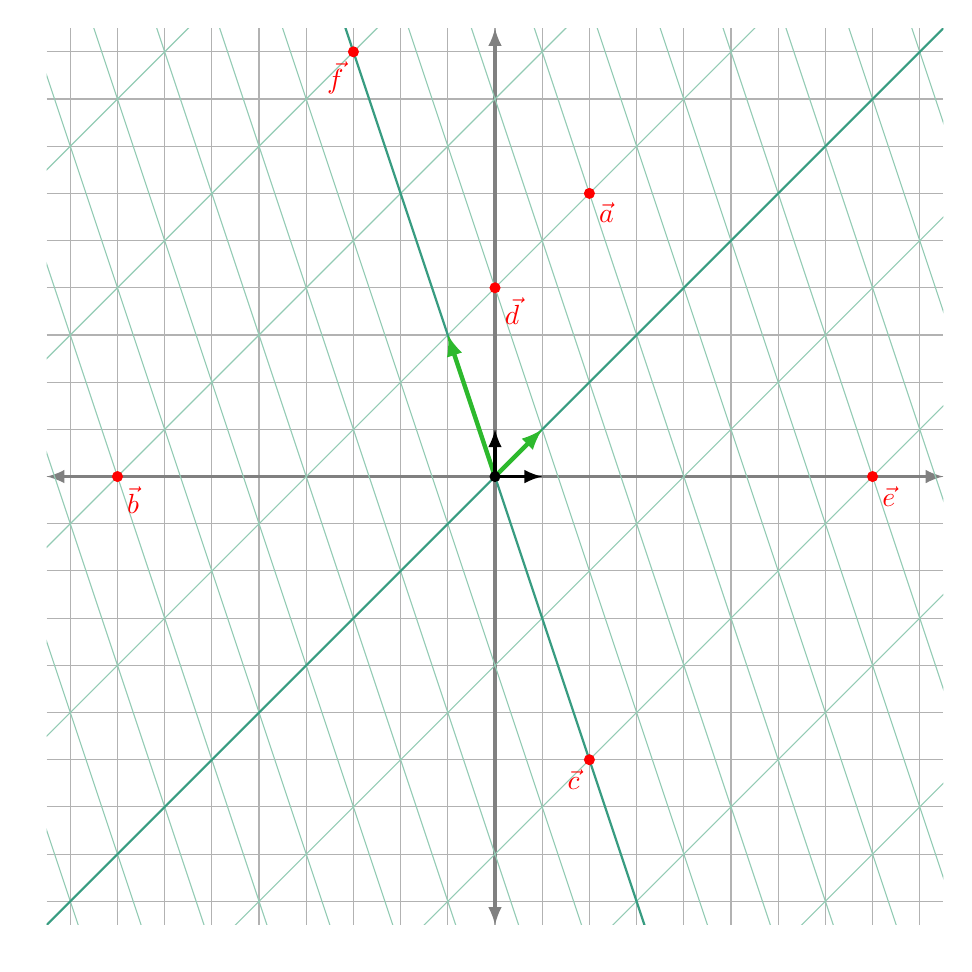
\begin{tikzpicture}[>=latex]
    \begin{axis}[scale=2,
		    axis equal image,
		    axis line style={draw=none},
		    tick style={draw=none},
		    yticklabels={,,},
		    xticklabels={,,},
		 xmin=-9.5,
		 xmax=9.5,
		 ymin=-9.5,
		 ymax=9.5,
		 major grid style={black!30!white},
                 xtick={-10,-9,...,11},
                 ytick={-10,-9,...,11},
                 grid=both]

		 \coordinate (A) at (-9.5, 0);
		 \coordinate (B) at (9.5, 0);
		 \coordinate (C) at (0, -9.5);
		 \coordinate (D) at (0, 9.5);
		\draw[<->, very thick, black!50!white] (A) -- (B);
		\draw[<->, very thick, black!50!white] (C) -- (D);
		

	    \foreach \ival in {-40,-36,...,40} {
	    	\edef\temp{\noexpand\draw[PineGreen!40!white] (-12,36+\ival) -- (12,-36+\ival);}
		\temp
	    	\edef\temp{\noexpand\draw[PineGreen!40!white] (-36,-36+\ival) -- (36,36+\ival);}
		\temp
	    }
	    \draw[PineGreen!80!white, thick] (-12,36) -- (12,-36) (-36,-36) -- (36, 36);
	    \draw[->, ultra thick, LimeGreen!90!black] (0,0) -- (1,1);
	    \draw[->, ultra thick, LimeGreen!90!black] (0,0) -- (-1,3);
	    \draw[->, very thick, black] (0,0) -- (0,1);
	    \draw[->, very thick, black] (0,0) -- (1,0);


	  	\fill[fill=black] (0,0) circle[radius=2pt];
	  	\fill[red] (2,6) circle[radius=2pt] node[below right] {$\vec a$};
	  	\fill[red] (-8,0) circle[radius=2pt] node[below right] {$\vec b$};
	  	\fill[red] (2,-6) circle[radius=2pt] node[below left] {$\vec c$};
	  	\fill[red] (0,4) circle[radius=2pt] node[below right] {$\vec d$};
	  	\fill[red] (8,0) circle[radius=2pt] node[below right] {$\vec e$};
	  	\fill[red] (-3,9) circle[radius=2pt] node[below left] {$\vec f$};
    \end{axis}
\end{tikzpicture}
\end{center}



\begin{enumerate}
	\item Write each point above in both the green and the black bases.
	\item Find a change-of-basis matrix $X$ that converts vectors from
		a green basis representation to a black basis representation. Find
		another matrix $Y$ that converts vectors from a black basis representation
		to a green basis representation.
	\item Let $T:\R^2\to\R^2$ be the linear transformation that stretches in the $y=-3x$ direction
		by a factor of $2$ and leaves vectors in the $y=x$ direction fixed.

		Describe what happens to the vectors $\vec u$, $\vec v$, and $\vec w$ when
		$T$ is applied given that 
		\[
			[\vec u]_{\mathcal G} = \mat{6\\1} \qquad 
			[\vec v]_{\mathcal G} = \mat{4\\-3} \qquad 
			[\vec u]_{\mathcal B} = \mat{-8\\-7}.
		\]
	\item When working with the transformation $T$, which basis do you prefer vectors be
		represented in?
\end{enumerate}
\end{iola}







%\section*{Span Again}
%	\question
%	Consider the system 
%		\begin{equation}\label{eq4bc}
%			\begin{array}{llll}
%				x&-y&-z &= 0\\
%				0x&+1y&+2z &= 0\\
%				3x&-3y&+3z &= 0
%			\end{array}
%		\end{equation}
%	which has the unique solution $(x,y,z)=(0,0,0)$.
%	\begin{parts}
%		\item Give vectors $\vec u,\vec v,\vec w$ so that the system \eqref{eq4bc}
%			corresponds to the vector equation $x\vec u+y\vec v+z\vec w = \vec 0$.
%		\item Is $\vec w\in\Span\{\vec u,\vec v\}$? If so, write it as a linear combination
%			of $\vec u$ and $\vec v$.
%	\end{parts}
%
%	The matrix $M$ is the non-augmented matrix corresponding to a homogeneous system of linear equations.
%	$M$ also corresponds to the vector equation $x\vec a+y\vec b+z\vec c=\vec 0$.  Further, we know
%	\[
%		\rref(M) = \mat{1&0&1\\0&1&-2\\0&0&0}.
%	\]
%	\begin{parts}[resume]
%		\item Give a solution to the vector equation $x\vec a+y\vec b+z\vec c=\vec 0$.
%		\item Is $\vec c\in\Span\{\vec a,\vec b\}$?  If so, write it as a linear combination
%			of $\vec a$ and $\vec b$.
%		\item Do you have enough information to tell if $\{\vec a,\vec b\}$ is linearly independent?  Why or why not?
%	\end{parts}
%
%\subsection*{Finding Linearly Independent Subsets}
%	\question
%	Suppose when you use an augmented matrix to solve
%	$a\vec u+b\vec v+c\vec w=\vec 0$ you have no free variables.
%	
%	\begin{parts}
%		\item Is $\{\vec u,\vec v,\vec w\}$ linearly independent?
%	\end{parts}
%	
%	Suppose when you use an augmented matrix to solve
%	$a\vec u+b\vec v+c\vec w=\vec 0$, the second column corresponds to a 
%	free variable.
%	
%	\begin{parts}[resume]
%		\item Is $\{\vec u,\vec v,\vec w\}$ linearly independent?
%		\item Is $\{\vec u,\vec w\}$ linearly independent?
%		\item Is $\{\vec u,\vec v\}$ linearly independent?
%	\end{parts}
%
%	\begin{definition}[Maximal Linearly Independent Subset]
%	Given a set of vectors $X$, a 
%	\emph{maximal linearly independent subset} of $X$ is a linearly independent
%	subset $V\subseteq X$ with the most possible vectors in it 
%	(i.e., if you took any subset of $X$ with more vectors, it would be linearly
%	dependent).
%	\end{definition}
%
%	\question
%	\begin{parts}
%		\item Give a maximal linearly independent subset, $T$, of
%		$\left\{\mat{a\\b\\c}:a,b,c\in \R\right\}$.
%		\item What is the size of $T$?
%	\end{parts}
%
%	\question
%	Consider the vectors
%	\[
%		\vec v_1=\mat{1\\2\\1}
%		\qquad
%		\vec v_2=\mat{-1\\-1\\-1}
%		\qquad
%		\vec v_3=\mat{0\\1\\0}
%		\qquad
%		\vec v_4=\mat{-1\\2\\0}
%		\qquad
%		\vec v_5=\mat{1\\-1\\1}
%	\]
%	and the matrices
%	\[
%		A=\mat{1&-1&0&-1&1\\ 2&-1&1&2&-1\\1 & -1&0&0&1}
%		\qquad \rref (A)
%		=\mat{1&0&1&0&-2\\0&1&1&0&-3\\0&0&0&1&0}.
%	\]
%	(Notice that the columns of $A$ are the vectors $\vec v_1,\ldots, \vec v_5$)
%
%	\begin{parts}
%		\item Is $V=\{\vec v_1,\vec v_2,\vec v_3,\vec v_4,\vec v_5\}$ linearly
%		independent?
%		\item Pick a maximal linearly independent subset of $V$.
%		\item Pick another (different) maximal linearly independent subset of $V$.
%		\item Give a basis for $\Span(V)$.
%		\item What is the dimension of $\Span(V)$?
%	\end{parts}
%
%	\newpage
%\section*{Matrices}
%	\question
%	\[
%		A=\mat{1&2\\3&1\\0&-1}
%		\qquad
%		B=\mat{-1&-1\\0&1\\1&-2}
%		\qquad
%		C=\mat{1&2&0\\-1&-1&-1}
%	\]
%	\begin{parts}
%		\item Write the shape of the matrices $A,B,C$ (i.e., for each one,
%		write the dimensions in $m\times n$ form).
%		\item List \emph{all} products between the matrices $A,B,C$ that are
%		defined. (Your list will be some subset of $AB,AC,BA,CA,BC,CB$.)
%		\item Compute $AC$ and $CA$.
%	\end{parts}
%
%	\question
%	\begin{parts}
%		\item If the matrices $X$ and $Y$ are both square $n\times n$ matrices,
%		does $XY=YX$?  Explain.
%		\item If the matrices $X$ and $Y$ are both square $n\times n$ matrices,
%		does $X+Y=Y+X$?  Explain.
%	\end{parts}
%
%	\question
%	The entries of a matrix are specified by (row,column) pairs of integers.  If
%	$a_{ij}$ is the $(i,j)$ entry of a matrix $A$, we may write $A=[a_{ij}]$.
%	\begin{parts}
%		\item Write the $2\times 2$ matrix $A$ with entries $a_{11} = 4$, $a_{12}=3$,
%			$a_{21} = 7$ and $a_{22}=9$.
%		\item Let $B=[b_{ij}]$ be the $3\times 3$ matrix where $b_{ij} = i+j$.  Write $B$.
%		\item Let $C=[c_{ij}]$ be the $3\times 4$ matrix where $c_{ij} = 0$ if $i=j$ and
%			$c_{ij}=1$ if $i\neq j$.
%	\end{parts}
%
%	\question
%	\begin{definition}
%		The \emph{transpose} of a matrix $A=[a_{ij}]$ is the matrix $A^{T}=[a_{ji}]$.
%	\end{definition}
%	Visually, the transpose of a matrix swaps rows and columns.
%
%	\[
%		A=\mat{1&1&2\\2&2&1}
%	\]
%	\begin{parts}
%		\item What is the shape of $A$ and $A^T$?
%		\item Write down $A^T$.
%	\end{parts}
%
%	$B$ and $D$ are $4\times 6$ matrices and $C$ is a $6\times 4$ matrix.
%
%	\begin{parts}[resume]
%		\item Does $(BC)^T=B^TC^T$? Explain.
%		\item Does $(B+D)^T=B^T+D^T$? Explain.
%		\item Compute $AA^T$ and $A^TA$ (where $A$ is the matrix defined earlier).
%		What do you notice?
%	\end{parts}
%
%	\question
%	\begin{definition}
%		A matrix $X$ is called \emph{symmetric} if $X=X^T$.  
%	\end{definition}
%	Symmetric matrices have many useful properties,
%	and have deep connections with orthogonality and eigenvectors (which we will get to later on).
%
%	\begin{parts}
%		\item Prove that if $W$ is a square matrix, then $V=W^TW+W+W^T$ is a symmetric
%		matrix.
%	\end{parts}
%
%	\question
%	\begin{definition}
%		A \emph{zero matrix} is a matrix whose entries are all zeros.
%		An \emph{identity matrix} is a square matrix whose diagonal
%		entries are $1$ and non-diagonal entries are $0$.
%	\end{definition}
%	We write the $m\times n$ zero matrix as $0_{m\times n}$ or just $0$ if the shape
%	is determined by context.  The $n\times n$ identity matrix is notated $I_{n\times n}$ or just
%	$I$ if the shape is determined by context.
%
%	Let $A=\mat{1&2&3\\4&5&6\\7&8&9}$.
%	\begin{parts}
%		\item Write down the $3\times 3$ identity matrix and the $3\times 3$ zero
%		matrix.
%		\item Compute $I_{3\times 3}A$, $AI_{3\times 3}$, $0_{3\times 3}A$,
%		and $A0_{3\times 3}$.
%		\item If we were to think of matrices as numbers, what numbers would the
%		zero matrix and the identity matrix correspond to?
%	\end{parts}
%
%	\question
%	\begin{parts}
%		\item Solve the matrix equation
%		\[
%			I_{4\times 4}\mat{x\\y\\z\\w} = \mat{2\\3\\1\\-1}.
%		\]
%	\end{parts}
%
%
%
%\newpage
%
%
%
%
%
%\newpage
%
%\section*{Orthogonality}
%	\begin{definition}[Orthogonal \& Orthonormal]
%		A set of vectors is \emph{orthogonal} if every pair of vectors
%		in the set is orthogonal.  A set of vectors is \emph{orthonormal}
%		if it is both an orthogonal set and every vector is a unit vector.
%	\end{definition}
%
%	\question
%	\[
%		\mathcal B=\{\vec b_1,\vec b_2\}\qquad\vec b_1=\mat{1/2\\\sqrt{3}/2}
%		\qquad \vec b_2=\mat{-\sqrt{3}/2\\1/2}
%	\]
%	The matrix $A=[\vec b_1|\vec b_2]$ takes vectors in the $\mathcal B$ basis
%	and rewrites them in the standard basis.
%	\begin{parts}
%		\item What does $A^{-1}$ do?
%		\item Find a matrix $B$ that takes vectors in the standard basis
%			and rewrites them in the $\mathcal B$ basis.
%		\item Write $\vec x=\mat{1\\2}$ in the $\mathcal B$ basis.
%		\item What is the relationship between $A$ and $B$?
%	\end{parts}
%
%	\begin{definition}[Orthogonal Matrix]
%		An \emph{orthogonal matrix} is a square matrix whose columns are
%		orthonormal (Yes, a better name would be orthonormal matrix, but that
%		is not the term the rest of the world uses).
%	\end{definition}
%
%	\question
%	Suppose $X=[\vec x_1|\vec x_2|\vec x_3|\vec x_4]$ is an orthogonal matrix.
%	\begin{parts}
%		\item What is the shape of $X$ (i.e., it is a what$\times$what matrix)?
%		\item Compute $X^TX$.
%		\item What is $X^{-1}$?
%	\end{parts}
%
%	\question
%	\[
%		Y=\mat{1&1&1&-1\\1&-1&-1&-1\\1&1&-1&1\\1&-1&1&1}
%	\]
%	\begin{parts}
%		\item Is $Y$ an orthogonal matrix?
%		\item Fix $Y$ so it is an orthogonal matrix.  Call the new matrix $X$.
%		\item Compute $X^{-1}$.
%		\item Compute $Y^{-1}$.
%		\item Compute $|\det(X)|$ and $|\det(Y)|$ (the absolute value of
%			the determinant of $X$ and $Y$).
%	\end{parts}
%
%	Matrix equations involving orthogonal matrices are easy to solve because the
%	inverse of an orthogonal matrix is so easy to compute!
%	
%	\question
%	Let $A=[\vec a_1|\vec a_2|\vec a_3|\vec a_4]$ be an orthogonal matrix.
%	\begin{parts}
%		\item Explain why 
%			$\vec x=\mat{\vec a_1\cdot \vec b\\
%				     \vec a_2\cdot \vec b\\
%			     	     \vec a_3\cdot \vec b\\
%			     	     \vec a_4\cdot \vec b}$ is a solution to $A\vec x=\vec b$.
%		\item Find scalars $a,b,c,d$ so $\vec b=a\vec a_1+b\vec a_2+c\vec a_3+d\vec a_4$
%			(your answers will have variables in them).
%	\end{parts}
%
%	Orthogonal matrices also allow us to compute projections quite easily.
%
%	\begin{definition}[Orthogonal Projection]
%		If $V$ is a subspace of $\R^n$, the \emph{projection}
%		(sometimes called the orthogonal projection) of $\vec x$ onto $V$
%		is the closest point in $V$ to $\vec x$. We notate the projection
%		of $\vec x$ onto $V$ as $\proj_V\vec x$.
%	\end{definition}
%
%	Projections are normally hard to compute and a priori might require some sort
%	of calculus-style optimization to find.  However, from geometry we know that 
%	if we travel from $\proj_V \vec x$ to $\vec x$, we should always trace out a path
%	perpendicular to $V$.  Otherwise, we could find a point in $V$ that was slightly closer
%	to $\vec x$, violating the definition of $\proj_V \vec x$.  Thus, orthogonality
%	will be our savior.
%
%	\question
%	Let $\mathcal S=\{\vec e_1,\vec e_2,\vec e_3\}$ be the standard basis.
%	\begin{parts}
%		\item If $\vec x=1\vec e_1+2\vec e_2+3\vec e_3$, find the projection of $\vec x$
%			onto the $xy$-plane.
%	\end{parts}
%	Suppose $\mathcal B=\{\vec b_1,\vec b_2,\vec b_3\}$ is an orthonormal basis for $\R^3$.
%	\begin{parts}[resume]
%		\item If $\vec y=3\vec b_1-2\vec b_2+2\vec b_3$, find the projection of $\vec y$
%			onto $\span\{\vec b_1,\vec b_3\}$.
%	\end{parts}
%	Suppose $\mathcal C=\{\vec c_1,\vec c_2,\vec c_3\}$ is a basis for $\R^3$ with
%	\[
%		\|\vec c_1\| = 
%		\|\vec c_2\| = 
%		\|\vec c_3\| = 1\qquad \vec c_1\cdot \vec c_2=0\qquad \vec c_1\cdot \vec c_3=0
%		\qquad \vec c_2\cdot \vec c_3=\sqrt{2}/2.
%	\]
%	\vspace{-.35in}
%	\begin{parts}[resume]
%		\item If $\vec z=5\vec c_1+2\vec c_2-\vec c_3$, find the projection of $\vec z$
%			onto $\span\left\{\vec c_1,\vec c_2\right\}$.
%	\end{parts}
%
%	\question
%	Let's put this all together.  
%	$\mathcal B=\left\{\mat{2\\1\\1},\mat{1\\-1\\-1},\mat{0\\1\\-1}\right\}$ is an
%	orthogonal basis for $\R^3$.  Let $\mathcal P$ be the plane defined
%	by
%	\[
%		0x+y-z=0.
%	\]
%	\begin{parts}
%		\item Write $\mathcal P$ in vector form (Hint: think about the vectors
%			listed in the $\mathcal B$ basis).
%		\item Find an orthonormal basis $\mathcal C=\{\vec c_1,\vec c_2,\vec c_3\}$
%			for $\R^3$ so $\mathcal P=\span\{\vec c_1,\vec c_2\}$.
%		\item Let $\vec x=\mat{1\\2\\3}$.  Find $\proj_{\mathcal P}\vec x$.
%	\end{parts}
%
%%\newpage
%\subsection*{Gram-Schmidt Orthogonalization}
%	We've seen how useful orthonormal bases are.  The incredible thing is that we can 
%	turn any basis into an orthonormal basis through a process called
%	Gram-Schmidt orthogonalization.
%
%	\question
%	Let $\vec a=\mat{1\\2}$ and $\vec b=\mat{3\\1}$.
%	\begin{parts}
%		\item Draw $\vec a$ and $\vec b$ and find $\vec w=\proj_{\vec b}\vec a$.
%		\item Add $\vec c=\vec a-\vec w$ to your drawing.  What is the angle between
%			$\vec c$ and $\vec b$.
%		\item Can you write $\vec a$ as the sum of two vectors, one in 
%			the direction of $\vec b$ and one orthogonal to $\vec b$?
%			If so, do it.
%	\end{parts}
%
%	\question
%	Let $\vec a=\mat{1\\2\\6}$ and $\vec b=\mat{1\\1\\-1}$.
%	\begin{parts}
%		\item Write $\vec a=\vec u+\vec v$ where $\vec u$ is parallel to
%			$\vec b$ and $\vec v$ is orthogonal to $\vec b$.
%		\item Find an orthonormal basis for $\span\{\vec a,\vec b\}$.
%	\end{parts}
%
%	With two vectors, making an orthonormal set without changing the span
%	is quite easy.  With more vectors, it is only slightly harder.
%
%	\begin{definition}[Gram-Schmidt Process]
%		The \emph{Gram-Schmidt} orthogonalization procedure
%		takes in a set of vectors and outputs a set of orthonormal vectors
%		with the same span.  The idea is to iteratively produce a set of
%		vectors where each new vector you produce is orthogonal to the previous vectors.
%
%		The algorithm is as follows: Let $\{ v_1,\ldots, v_n\}$ be a set of 
%		vectors.  Produce a set $\{ v_2',\ldots, v_n'\}$ that is orthogonal
%		to $ v_1$ by subtracting off the respective projections
%		of $ v_2,\ldots, v_n$
%		onto $ v_1$.  Next, produce a set $\{ v_3'',\ldots, v_n''\}$
%		orthogonal to both $ v_1$ and $ v_2'$ by subtracting off the
%		respective projections
%		onto $ v_2'$.  Continue this process until you have a set
%		$V=\{ v_1, v_2', v_3'', v_4''',\ldots\}$ that is orthogonal.
%		Finally, normalize $V$ so all vectors have unit length.
%	\end{definition}
%
%	\question
%	Let $\vec x_1=\mat{1\\-1\\-1\\1}$, $\vec x_2=\mat{2\\1\\0\\1}$, and 
%	$\vec x_3=\mat{2\\2\\1\\2}$.
%	\begin{parts}
%		\item Use the Gram-Schmidt procedure to find an orthonormal basis for 
%			$\span\{\vec x_1,\vec x_2,\vec x_3\}$.
%		\item Find an orthonormal basis $\mathcal V=\{\vec v_1,\vec v_2,\vec v_3,\vec v_4\}$
%			for $\R^4$ so that $\span\{\vec v_1,\vec v_2,\vec v_3\}=
%			\span\{\vec x_1,\vec x_2,\vec x_3\}$.
%	\end{parts}
%	Let $R=\mat{1&-1&-1&1\\2&1&0&1\\2&2&1&2}$.
%	\begin{parts}[resume]
%		\item Find an orthonormal basis for the row space of $R$.
%		\item Find the null space of $R$ (Hint, you've already done the work, so
%			there is no need to row reduce).
%	\end{parts}
%
%	\question
%	Let
%	\[
%		\vec y_1=\mat{1\\1\\2}\qquad 
%		\vec y_2=\mat{-1\\-1\\2}\qquad
%		\vec y_3=\mat{1\\1\\6}.
%	\]
%	\begin{parts}
%		\item Find an orthonormal basis $\mathcal W$ so that $\span\mathcal W=
%			\span\{\vec y_1,\vec y_2,\vec y_3\}$.
%	\end{parts}
%
%	\begin{definition}[Orthogonal Complement]
%		The \emph{orthogonal complement} of a subspace $V$ is written
%		$V^\perp$ and defined as
%		\[
%			V^\perp=\{\vec x:\vec x\text{ is orthogonal to }V\}.
%		\]
%		\vspace{-.2in}
%	\end{definition}
%
%	\begin{parts}[resume]
%		\item Find the orthogonal complement of $\span \mathcal W$.
%		\item Write $\vec v=\mat{1\\0\\1}$ in the form $\vec v=\vec r+\vec n$ where 
%			$\vec r\in\span\mathcal W$ and $\vec n\in(\span \mathcal W)^\perp$.
%	\end{parts}
%
%
%\subsection*{$QR$ Decomposition}
%
%	\begin{definition}[$QR$ Decomposition]
%		For a matrix $A$, we can rewrite $A=QR$ where $Q$ is an
%		orthogonal matrix and $R$ is an upper triangular matrix.  Writing
%		$A$ as $QR$ is called the \emph{$QR$ decomposition} of $A$.
%	\end{definition}
%
%	\question
%	Suppose $A,B,C$ are square matrices and $C=AB$.
%	\begin{parts}
%		\item How do the column spaces of $A$ and $C$ relate?
%		\item How do the column spaces of $B$ and $C$ relate?
%	\end{parts}
%
%	\question
%	$\mathcal V=\{\vec v_1,\vec v_2,\vec v_3\}$ forms a basis for $\R^3$.
%	When we apply the Gram-Schmidt process to $\mathcal V$, we get
%	\[
%		\begin{array}{rl}
%			q_1' &=\vec v\\
%			q_2' &= \vec v_2-\frac{1}{2}\vec v_2\\
%			q_3' &= \vec v_3-\vec v_1+2\vec v_2
%		\end{array}
%	\]
%	form an orthogonal set.  Normalizing we get
%	\[
%		\begin{array}{rl}
%			\vec q_1 &= 2q_1'\\
%			\vec q_2 &= 3q_2'\\
%			\vec q_3 &=\frac{1}{2}q_3'
%		\end{array}
%	\]
%	form an orthonormal set.
%	\begin{parts}
%		\item Write $\vec v_1$ as a linear combination of $\vec q_1,\vec q_2,\vec q_3$.
%		\item Write $\vec v_2$ as a linear combination of $\vec q_1,\vec q_2,\vec q_3$.
%		\item Write $\vec v_3$ as a linear combination of $\vec q_1,\vec q_2,\vec q_3$.
%	\end{parts}
%	Define $A=[\vec v_1|\vec v_2|\vec v_2]$ and $Q=[\vec q_1|\vec q_2|\vec q_3]$.
%	\begin{parts}[resume]
%		\item Find a matrix $R$ so that $A=QR$.
%	\end{parts}
%	
%	We've just discovered one process to find the $QR$ decomposition of a matrix.
%	It's really as simple as doing Gram-Schmidt and keeping track of your coefficients.
%	Now, we have another way to the matrix equation $A\vec x=\vec b$.  If we do a $QR$
%	decomposition and exploit the fact that $Q^{-1}=Q^T$, we have
%	\[
%		A\vec x=QR\vec x=\vec b\qquad\implies\qquad R\vec x=Q^T\vec b
%	\]
%	and $R$ is a triangular matrix, so we can just do back substitution! (It turns
%	out that if you solve systems this way, there is less rounding error than if you
%	use row reduction.)
%
%\subsection*{Symmetric Matrices}
%	When you're new to Linear Algebra, learning lots of new concepts and algorithms,
%	it's sometimes hard to grasp the significance of certain properties of a matrix.
%
%	Symmetric matrices are easy to forget at first, but they have many profound 
%	properties (not to mention they are one of the key concepts of Quantum Mechanics).
%
%	\question
%	Let $A$ be a symmetric matrix and let $\vec v$ be an eigenvector with eigenvalue
%	3 and $\vec w$ be an eigenvector with eigenvalue 4.  Note, for this problem,
%	we are thinking of $\vec v$ and $\vec w$ as column vectors.
%	\begin{parts}
%		\item Write $A\vec v$, $\vec v^TA^T$, $\vec v^TA$, $A\vec w$, $\vec w^TA^T$, 
%		and $\vec w^TA$ in terms of $\vec v$, $\vec w$ and scalars.
%		\item How do $\vec v^T\vec w$ and $\vec w^T\vec v$ relate?
%		\item What should $\vec v^TA\vec w$ be in terms of $\vec v^T$ and
%			$\vec w$? (Note, you could compute $(\vec v^TA)\vec w$
%			or $\vec v^T(A\vec w)$.  Better do both to be safe).
%		\item What can you conclude about $\vec v^T\vec w$?  How about
%			$\vec v\cdot \vec w$?
%	\end{parts}
%
%	We've just deduced that all eigenspaces of a symmetric matrix are orthogonal! On
%	top of that, symmetric matrices always have a basis of eigenvectors.  That means
%	that not only can you always diagonalize a symmetric matrix, but you can 
%	\emph{orthogonally} diagonalize a symmetric matrix. (i.e. if $A$ is symmetric,
%	then $A=QDQ^T$ where $Q$ is orthogonal and $D$ is diagonal).  This is like the 
%	best of all worlds in one!
%
%
%
%\section*{Systems of Linear Equations}
%	
%	\emph{Linear equations} are equations only involving variables, 
%	multiplication by constants, and addition/subtraction.  \emph{Systems}
%	of equations are sets of equations that share common variables.
%
%	\question
%	Consider the system
%	\begin{equation}\label{eq2}
%		\begin{array}{rcrl}
%			x &-&y &= 2\\
%			2x &+&y &= 1
%		\end{array}
%	\end{equation}
%
%	\begin{parts}
%		\item Draw the lines in (\ref{eq2}) on the same coordinate plane.
%		\item Algebraically solve the system (\ref{eq2}).  What does this 
%		solution represent on your graph?
%	\end{parts}
%	
%	\question
%	Let $L$ be the line given by $x-y=2$.
%	\begin{parts}
%		\item Write an equation of a line that doesn't intersect $L$.
%		\item Write an equation of a line that intersects $L$ in 
%		\begin{enumerate}
%			\item one place.
%			\item infinitely many places
%			\item exactly two places
%		\end{enumerate}
%		or explain why no such equation exists.
%		\item For each equation you came up with, solve the system algebraically.
%		How can you tell algebraically how many solutions there are?
%	\end{parts}
%
%\subsection*{The Row Reduction Algorithm}
%
%	\question
%	\begin{parts}
%		\item Solve the system
%		\begin{equation}\label{eq3}
%			\begin{array}{rcrcrl}
%				x&-&y&-&2z &= -5\\
%				2x&+&3y&+&z &= 5\\
%				0x&+&2y&+&3z &= 8
%			\end{array}
%		\end{equation}
%		any way you like.
%
%		\item Use an augmented matrix to solve the system (\ref{eq3}).
%	\end{parts}
%
%	The system (\ref{eq3}) can be interpreted in two ways (and switching between these 
%	interpretations when appropriate is one of the most powerful tools of Linear 
%	Algebra).  We can think of solutions to (\ref{eq3})
%	as the intersection of three planes, or we can interpret the solution
%	as coefficients of a linear combination.
%
%	\begin{parts}[resume]
%		\item Rewrite (\ref{eq3}) as a vector equation of the form
%		\[
%			x\vec v_1+y\vec v_2+z\vec v_3 = \vec p
%		\]
%		where $x,y,z$ are interpreted as scalar quantities.
%
%		\item If $(x,y,z)$ is a solution to (\ref{eq3}), explain how to get from the
%		origin to $\vec p$ using only $\vec v_1, \vec v_2, \vec v_3$.
%		\item If $(x,y,z)$ is a solution to \eqref{eq3}, is $\vec p\in\Span\{\vec v_1,\vec v_2,\vec v_3\}$?
%	\end{parts}
%
%	\question
%	Consider the augmented matrix
%	\[
%		A=\left[\begin{array}{ccc|c}
%			1 & 2 & -1 & -7\\
%			0 & 2 & 3 & 9\\
%			0 & 0 & 1 & 1
%		\end{array}\right].
%	\]
%	\begin{parts}
%		\item Write the system of equations corresponding to $A$.
%		\item Solve the system of equations corresponding to $A$.
%	\end{parts}
%
%\subsection*{Infinite Solutions}
%	\question
%	Consider the system
%	\begin{equation}\label{eq4}
%		\begin{array}{rcrl}
%			x&+&2y &= 3\\
%			2x&+&4y &= 6
%		\end{array}
%	\end{equation}
%
%	\begin{parts}
%		\item How many solutions does (\ref{eq4}) have?
%		\item Write the solutions to (\ref{eq4}) in vector form.
%		\item What happens when you use an augmented matrix
%		to solve (\ref{eq4})?
%	\end{parts}
%
%
%\subsection*{Free Variables}
%	\question
%	Suppose the row-reduced augmented matrix corresponding to 
%	a system is
%	\[
%		B=\left[\begin{array}{cc|c}
%			1 & 2 & 3\\
%			0 & 0 & 0
%		\end{array}\right].
%	\]
%	After reducing, we have 1 equation and 2 unknowns, so we can make
%	$2-1=1$ choices when writing a solution.  Let's make the
%	choice $y=t$.
%	
%	\begin{parts}
%		\item With the added equation $y=t$, solve the
%		system represented by $B$.
%	\end{parts}
%
%	\question
%	Consider the system given by the augmented matrix
%	\[
%		C=\left[\begin{array}{ccccc|c}
%			1&0&1&2&0&-1\\
%			0&1&1&0&0&3\\
%			0&0&0&0&1&4
%		\end{array}\right].
%	\]
%	and call the variables in this system $x_1,x_2,
%	x_3,x_4,x_5$.
%
%	\begin{parts}
%		\item Write the system of equations represented by $C$.
%		\item Identify how many choices you can make when writing
%		down a solution corresponding to $C$.
%		\item Add one equation (of the form $x_i=t$ or $x_j=s$, etc.)
%		for each choice you must make when solving the system.
%		\item Write in vector form all solutions to $C$.
%	\end{parts}
%
%	\question
%	\begin{parts}
%		\item An unknown system $U$ is represented by an augmented
%		matrix with 4 rows and 6 columns.  What is 
%		the minimum number of
%		free variables solutions to $U$ will have?
%		\item An unknown system $V$ is represented by an augmented
%		matrix with 6 rows and 4 columns.  What is 
%		the minimum number of
%		free variables solutions to $V$ will have?
%	\end{parts}
%	
%	\question
%	\begin{definition}[Homogeneous]
%		A system is called \emph{homogeneous} if all equations equal $0$.
%	\end{definition}
%
%		Let $A$ be an unknown system of $3$ equations and $3$ variables and suppose
%		 $(x,y,z)=(1,2,1)$ and
%		$(x,y,z)=(-1,1,1)$ are solutions to $A$.
%	\begin{parts}
%		\item Can you produce another solution
%		to the system?
%
%		\item  Can you
%		produce a solution to the homogeneous version of $A$ (the version of $A$ where every
%		equation equals 0)?
%
%		\item Suppose when you use an augmented matrix to solve the system $A$, you only have 
%		one free variable.  Could $A$ be homogeneous?  Can you produce all solutions to the system $A$?
%	\end{parts}
%







\end{document}
